\documentclass[a4paper]{article}
\title{\Huge{\textsc{Word Embeddings with Multiple Word Prototypes}}}
\usepackage[margin=3cm]{geometry}
\usepackage{graphicx}
\usepackage{wrapfig}
\usepackage{caption}
\usepackage{amsmath}
\usepackage{subcaption}
\usepackage[export]{adjustbox}
\usepackage{enumerate}
\usepackage{url}
\usepackage{authblk}
\usepackage{float}
\usepackage{wrapfig}
\usepackage{setspace}
\usepackage{mdframed}
\usepackage{booktabs}
\usepackage{ragged2e}

\def\changemargin#1#2{\list{}{\rightmargin#2\leftmargin#1}\item[]}
\let\endchangemargin=\endlist 

\DeclareMathSizes{10}{10}{10}{10}
\begin{document}

    \newgeometry{left=4cm,right=4cm,top=4cm,bottom=6cm}
	\begin{titlepage}
	    \begin{center}
	        \vspace*{1cm}
	        
	        {\huge{\textsc{Evolutionary Algorithms for Infinite Prisoner's Dilemma}}\\}
	        \vspace{8mm}
	        {\large{Nishant Rai}}\\
			\vspace{3mm}
			
			{\normalsize{Department of Computer Science and engineering\\}}
	        \vspace{4mm}
        	\vspace{7mm}
	        \textbf{Abstract\\}
        	\vspace{4mm}
        	\noindent
{\justifying{The project deals with the problem of computing successful strategies for Infinite Prisoner's dilemma. We propose multiple algorithms to compute good strategies which perform well against a set of baseline algorithms (Including the extremely simple yet effective 'Tit for Tat'). We discuss Axelrod's Tournament and use a similar setup to decide the effectiveness of the computed strategies. The result section shows the superiority of the strategies computed using them.} \par}
			\vfill
			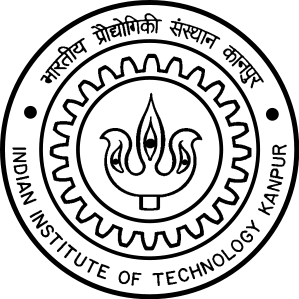
\includegraphics[width=0.25\textwidth]{iitklogo.png}\\[0.1in]
            \vspace{3mm}
            \normalsize{Under the guidance of Dr. Vimal Kumar\\}
            \vspace{1mm}
            {Indian Institute of Technology, Kanpur}
	    \end{center}
	\end{titlepage}
	\restoregeometry

	\tableofcontents
	
	\pagebreak	
	
	\section{Introduction}
	
	\section{Related Work}
	
	\section{Axelrod's Tournament}
	
	\subsection{Features of Successful Strategies}

	\subsection{Axelrod Strategies}	
	
	\section{Motivation}
	
	\section{Proposed Algorithms}
	
	\subsection{Axelrod Strategies using Evolutionary Algorithms}

	\subsection{Reinforcement Learning for Adaptive Strategies}
	
	\section{Experiments}
	
	\subsection{Tournament Setup}
	
	\subsection{Baseline Strategies}

	\section{Results}
	
	\section{Observations}
	
	\subsection{Effect of Memory on Strategies}	
		
	\section{Future Work}
			
\end{document}


